\section{Application}
\subsection{Lancement de l'application}

	\begin{frame}
	\frametitle{Application}
	\framesubtitle{Ecran de chargement de l'application}
	
	\end{frame}
	
	
	\begin{frame}
	\frametitle{Application}
	\framesubtitle{Ecran d'accueil}
	
	\end{frame}
	
	\begin{frame}
	\frametitle{Application}
	\framesubtitle{Les menus}
	
	\end{frame}
	
\subsection{Editeur de cartes}

	\begin{frame}
	\frametitle{Application}
	\framesubtitle{Gestion des ressources}
	
	
	\end{frame}

	\begin{frame}
	\frametitle{Application}
	\framesubtitle{Création ou chargement d'une carte}
	
	\end{frame}
	
	\begin{frame}
	\frametitle{Application}
	\framesubtitle{Moteur de rendu cartes}
	
	\end{frame}
	
	
	\begin{frame}
	\frametitle{Application}
	\framesubtitle{Editeur de cartes}
	
	\end{frame}
	
	\begin{frame}
	\frametitle{Application}
	\framesubtitle{Outils}
	
	\end{frame}
	
	\begin{frame}
	\frametitle{Application}
	\framesubtitle{Exemple de carte}
	
	\end{frame}
	
	\begin{frame}
	\frametitle{Application}
	\framesubtitle{Possibilités finales}
	
	\end{frame}

\subsection{Jeu}
	
	\begin{frame}
	\frametitle{Application}
	\framesubtitle{Création d'une partie solitaire}
	
		\begin{tabular}{cc}
			\begin{minipage}{5cm}
				Création d'une partie solitaire
				\begin{enumerate}
					\item Choix de la carte
					\item Type de la partie
					\item Difficulté des ennemis
					\item Nombre d'ennemis
					\item Temps de la partie
					\item Retourner à l'écran d'accueil
					\item Créer la partie
				\end{enumerate}
			\end{minipage} &
			\begin{minipage}{7cm}
				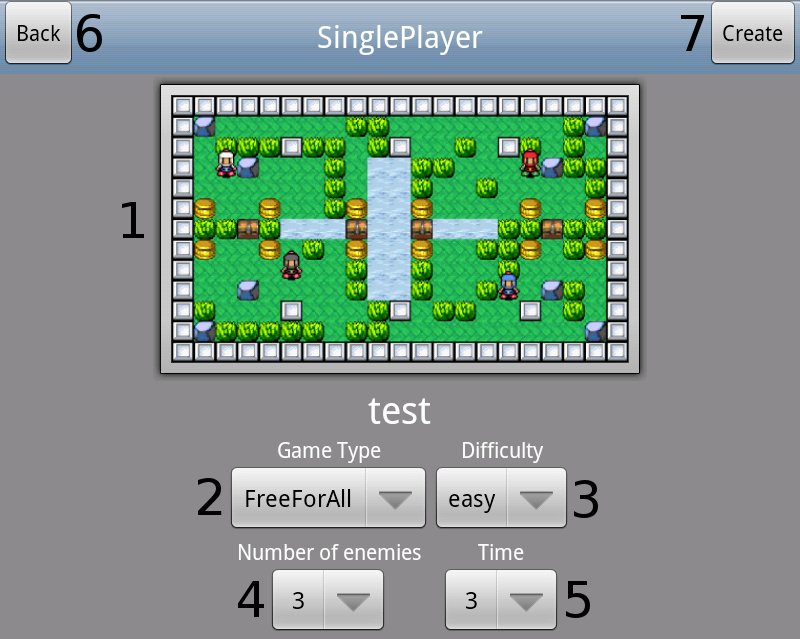
\includegraphics[width=6cm]{img/singleplayerbis.png} 
			\end{minipage}\\
		\end{tabular}
	
	\end{frame}
	
	\begin{frame}
	\frametitle{Application}
	\framesubtitle{Intelligence artificielle}
	
		\begin{tabular}{cc}
			\begin{minipage}{4cm}
				Niveaux de difficulté
				\begin{enumerate}
					\item Facile
					\item Moyen
					\item Difficile
				\end{enumerate}
			\end{minipage} &
			\begin{minipage}{6cm}
				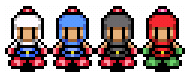
\includegraphics[width=6cm]{img/bots.png} 
			\end{minipage}\\
		\end{tabular}
	
	\end{frame}
	
	\begin{frame}
	\frametitle{Application}
	\framesubtitle{Pathfinding}
	
		\begin{tabular}{cc}
			\begin{minipage}{5cm}
				Algorithme A*
				\begin{enumerate}
					\item Heuristique (de Manatan)
					\item Coût de deplacement
					\item Premier chemin trouvé
					\item Rapidité (Dijskra)
				\end{enumerate}
			\end{minipage} &
			\begin{minipage}{5cm}
				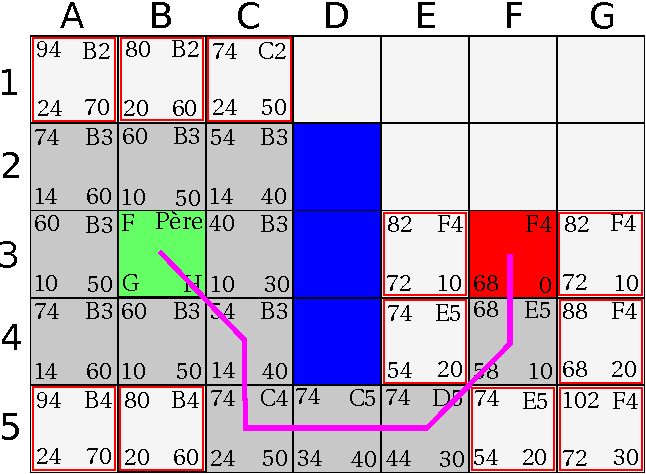
\includegraphics[width=6cm]{img/astar.png} 
			\end{minipage}\\
		\end{tabular}
	
	\end{frame}
	
	\begin{frame}
	\frametitle{Application}
	\framesubtitle{Pathfinding}
	
		\begin{tabular}{cc}
			\begin{minipage}{5cm}
				Algorithme de parcours en largeur
				\begin{enumerate}
					\item Pas de case d'arrivé necessaire
					\item Tous les chemins possibles
					\item Premier chemin trouvé
					\item Rapidité
				\end{enumerate}
			\end{minipage} &
			\begin{minipage}{5cm}
							\begin{center}
				\begin{tabular}{|c|c|c|c|c|c|c|} \hline
				\rowcolor{gray}  &  &                    &  &                  &  &                   \\\hline
				\cellcolor{gray} & \cellcolor{orange}1 $\leftarrow$ & \cellcolor{green}1 $\leftarrow$                   &&                && \cellcolor{gray} \\\hline
				\cellcolor{gray} & \cellcolor{orange}1 $\leftarrow$ & \cellcolor{gray}   & \cellcolor{gray} & \cellcolor{gray} &&	\cellcolor{gray} \\\hline
				\cellcolor{gray} & \cellcolor{orange}1 $\leftarrow$ & \cellcolor{orange}1 & \cellcolor{orange}1 $\rightarrow$ & \cellcolor{red}O                 && \cellcolor{gray} \\\hline
				\cellcolor{gray} & \cellcolor{orange}1 $\leftarrow$ & \cellcolor{gray}   & \cellcolor{gray} & \cellcolor{gray} && \cellcolor{gray} \\\hline
				\cellcolor{gray} & \cellcolor{red}O &                  &  &                && \cellcolor{gray} \\\hline
				\cellcolor{gray} && \cellcolor{gray}   && \cellcolor{gray} &&	\cellcolor{gray} \\\hline
				\cellcolor{gray} &&                  &&                && \cellcolor{gray} \\\hline
				\rowcolor{gray}  &  &                    &  &                  &  & \\\hline
				\end{tabular}
			\end{center}
			\end{minipage}\\
		\end{tabular}	
	
	\end{frame}
	
	\begin{frame}
	\frametitle{Application}
	\framesubtitle{Moteur de rendu}
	
		\begin{tabular}{ccccc}
			\begin{minipage}{3cm}
				\begin{center}
					Image
				\end{center}		
			\end{minipage} & &
			\begin{minipage}{2cm}
				\begin{center}
					Hashmap
				\end{center}
			\end{minipage} & &
			\begin{minipage}{3cm}
				\begin{center}
					Resultat
				\end{center}
			\end{minipage}\\
			\begin{minipage}{3cm}
				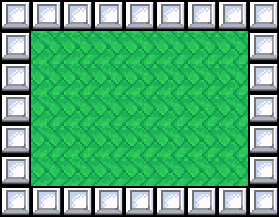
\includegraphics[width=3cm]{img/bitmap.png}
			\end{minipage} & + &
			\begin{minipage}{2cm}
				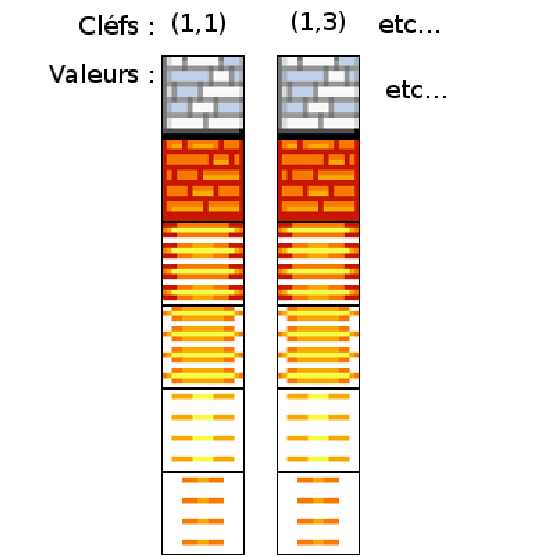
\includegraphics[width=3cm]{img/hashmap.png} 
			\end{minipage} & = &
			\begin{minipage}{3cm}
				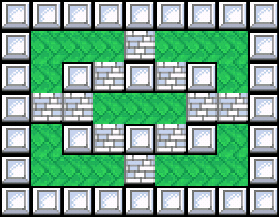
\includegraphics[width=3cm]{img/map.png} 
			\end{minipage}\\
		\end{tabular}
	
	\end{frame}
	
	\begin{frame}
	\frametitle{Application}
	\framesubtitle{Moteur Physique}
	
	\end{frame}
	
	\begin{frame}
	\frametitle{Application}
	\framesubtitle{Multitouch}
	
	\end{frame}
	
	\begin{frame}
	\frametitle{Application}
	\framesubtitle{Menu}
	
			\begin{tabular}{cc}
			\begin{minipage}{4cm}
				Menu
				\begin{enumerate}
					\item Reprendre
					\item Options
					\item Redemarrer
					\item Quitter
				\end{enumerate}
			\end{minipage} &
			\begin{minipage}{7cm}
				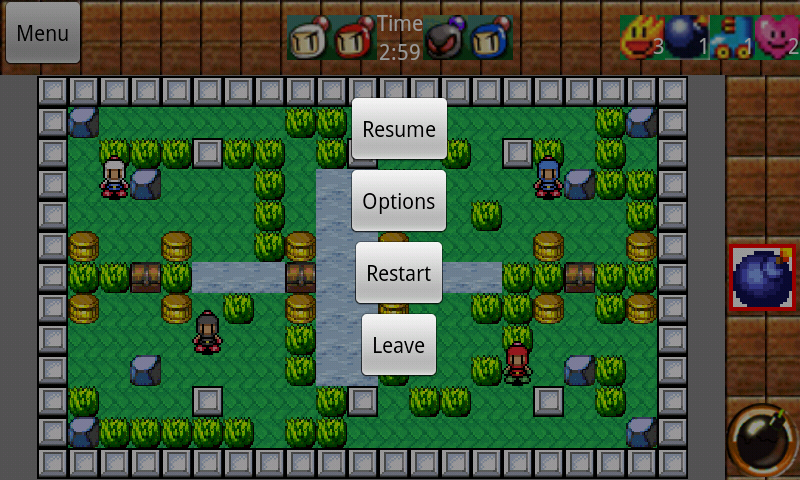
\includegraphics[width=7cm]{img/menusolo.png} 
			\end{minipage}\\
		\end{tabular}
	
	\end{frame}


\subsection{Reseau}